\documentclass[12pt]{article}

\usepackage{enumitem}
\usepackage[right=20mm, left=20mm]{geometry}
\usepackage{type1cm}
\usepackage{amssymb}
\usepackage[fleqn]{amsmath}
\usepackage{tikz}
\usepackage{multicol}
\usepackage{makecell}
\setlength{\columnsep}{1pt}
\usepackage{pgfplots}
\usepackage{float}
\usepackage{caption}
\usepackage{subcaption}
% \usepackage{subfig}
\usepackage{graphicx}

\usepackage{indentfirst}
\usepackage{lastpage}  
\usepackage{fancyhdr}
\pagestyle{fancy}

\usepackage[unicode=true,pdfusetitle,
 bookmarks=true,bookmarksnumbered=false,bookmarksopen=false,
 breaklinks=false,pdfborder={0 0 1},backref=false,colorlinks=false]
 {hyperref}

\makeatletter
\newenvironment{myalign*}{\ifvmode\else\hfil\null\linebreak\fi
  \hspace*{-\leftmargin}\minipage\textwidth
  \setlength{\abovedisplayskip}{0pt}%
  \setlength{\abovedisplayshortskip}{\abovedisplayskip}%
  \start@align\@ne\st@rredtrue\m@ne}%
{\endalign\endminipage\linebreak}

% Paper size
\topmargin -10mm
\textwidth 170mm
% \oddsidemargin -5mm
% \evensidemargin -5mm
\textheight 220mm

% Font setting
\usepackage{xeCJK}
% \setCJKmainfont{Noto Sans TC}
\setCJKmainfont{kaiu.ttf}


\renewcommand{\footnotesize}{\normalsize} 
\renewcommand{\headrulewidth}{0pt}
\renewcommand{\footrulewidth}{0pt}

\lhead{}
\chead{「Slide Talker 頭部畫面融合演講影片」 - 提升觀看教學影片效果}
\rhead{}

\lfoot{}
\cfoot{}
\rfoot{ 共 \pageref{LastPage} 頁 第  \thepage   頁} 

\makeatletter

\begin{document}
\date{}
\usetikzlibrary{automata, positioning, arrows}
% \maketitle
\tikzset{every state, accepting/.style={double distance=2pt}}
\captionsetup[figure]{labelfont={bf},name={圖},labelsep=period}

\noindent
\textbf{參賽隊名:} CJC\_club \\
\textbf{作品名稱:} 「Slide Talker 頭部畫面融合演講影片」 - 提升觀看教學影片效果

\begin{enumerate}
  \item 作品簡介
    \begin{enumerate}[label=\Alph*.]
      \setlength{\parindent}{2em}
      \item 創作動機與背景
        \par 在現今數位時代,影片已成為一種主要的學習和教學媒介,此外,因應疫情而出現的遠距教學也使得教學方式從實體轉為網路影片。然而,相較於與講者面對面的實體上課或演講,
        在觀看影片時,較容易分心或失去專注力。根據 Barbara 等人研究\cite{ref}指出,若影片有講師演講的畫面,可以提高觀眾的專注力。然而,要拍攝此種教學影片成本相對較高,包括架設專業的攝影器材和音響設備,以及錄製過程中可能面臨的錄影失敗風險。
        \par 因此,我們需要尋找一種成本較低且效果顯著的方法,使得製作教學影片變得更容易,同時提供觀眾更好的觀看體驗。
      \item 研究問題與專業領域
        \par 我們發現現今教學影片兩個主要問題:
        \begin{enumerate}[label=(\arabic*)]
          \item 觀眾專注力不足:在觀看教學影片時,觀眾容易分心或失去專注力,這影響了學習效果。
          \item 教學影片製作成本高:傳統的教學影片製作需要昂貴的攝影器材和專業的錄製設備,這使得製作教學影片門檻提高。
        \end{enumerate}
        \par 基於以上問題,本系統跨足教育領域,通過改進講師的教學影片製作方式,幫助講師以最小的成本實現預期的教學效果,從而提高觀眾的學習體驗和效果。
      \item 作品目的及解決問題
        \par 我們的作品旨在提供一個簡單易用的平台,讓講者能夠輕鬆地將自己的頭像畫面加入演講影片中,以改善觀眾的專注力和學習效果。講者可以上傳自己的頭像照片,並將其嵌入到演講影片中的適當位置。提供觀眾更優質的觀看體驗,同時降低製作成本,促進更有效的學習和教學。
      \item 創新創意
        \begin{enumerate}[label=(\arabic*)]
          \item 增強觀眾專注力:現在從Youtube影音平台中可以看到許多教學影片,但很多都是只有投影片及講師的聲音。因此我們通過將演講者的頭像演講畫面嵌入到演講影片中,觀眾在觀看影片時同時看到演講者的真實面容以及情緒表現,可以更好地理解和體驗演講的內容。
          \item 簡化製作過程:一般來說,若需要拍攝帶有頭像的高品質影片,需要有專業的攝影設備、燈光等,也需要克服面對鏡頭的恐懼。我們的平台提供了一個簡單易用的製作工具,只需要上傳操作簡報的影片及大頭照,就能夠按照影片的聲音及頭像,生成出繪聲繪影的演講影片。
        \end{enumerate}
      \item 主要功能
        \par 我們通過構建Web應用程序,講者只需提供演講影片和大頭照,並選擇生成的頭部模擬影像的設定,即可透過機器學習模型生成一個結合了以演講者大頭照為基礎的頭部模擬影像,並將其貼合至原演講影片中,最後呈現一部帶有演講者頭部畫面的演講影片。講者可以提供電子信箱,當影片生成完畢後會透過電子郵件通知講者。
      \item 實用性及預期之貢獻
        \par 我們的作品提供一個簡單快速的方式,讓講者省去大量成本的情況下提升影片的教學品質。無論是想要做程式教學、投資股票,甚至是電影解說都能透過我們的平台低成本快速做出高品質的影片,能夠應用在學校、線上教學及自媒體等。
        \par 這樣的技術可以幫助影片觀看者更好地專注於演講內容,減少分心和提高學習效果。無論是學生、教育工作者、還是任何需要進行教學或知識分享的專業人士,都可以受益於這項技術。
    \end{enumerate}
  \item 系統分析與設計\\
    需求分析:
    \begin{enumerate}[label=\Alph*.]
      \item 功能性需求:
        \begin{enumerate}
          \item 上傳資料功能
            \begin{enumerate}[label=(\arabic*)]
              \item 使用者能夠上傳錄製好的演講影片,包含投影片和音訊。
              \item 使用者能夠上傳一張照片作為頭部模擬。
            \end{enumerate}
          \item 影像合成功能
            \begin{enumerate}[label=(\arabic*)]
              \item 提供頭部模擬影像的參數調整功能,如位置、形狀等。
              \item 機器學習模型能夠根據提供的照片生成頭部模擬影像。
              \item 將頭部模擬影像與原影片合併。
            \end{enumerate}
          \item 通知功能
            \begin{enumerate}[label=(\arabic*)]
              \item 使用者能夠設定個人電子郵件
              \item 影片生成後將會寄信通知使用者
            \end{enumerate}
        \end{enumerate}
      \item 非功能性需求:
        \begin{enumerate}
          \item 使用性需求
            \begin{enumerate}[label=(\arabic*)]
              \item 清晰且直觀的使用者界面,使使用者能夠輕鬆上手。
              \item 提供指示和說明,協助使用者完成相關操作。
            \end{enumerate}
          \item 效能需求
            \begin{enumerate}[label=(\arabic*)]
              \item 能夠同時接受 100 人發出請求,並使用排隊來限制請求數。
              \item 高效處理和合併影片,確保生成的最終演講影片具有流暢和一致的品質。
              \item 影片及大頭照只能上傳 1024 MB以下。
            \end{enumerate}
          \item 安全性需求
            \begin{enumerate}[label=(\arabic*)]
              \item 考慮使用者的資料安全和隱私保護,確保作品在資料處理和傳輸過程中具備適當的安全措施。
            \end{enumerate}
          \item 錯誤處理
            \begin{enumerate}[label=(\arabic*)]
              \item 良好的系統穩定性和可靠性,完善的錯誤處理,避免崩潰或故障情況。
              \item 針對使用者輸入做資料驗證。
              \item 若有錯誤訊息將完整記錄log。
            \end{enumerate}
        \end{enumerate}
    \end{enumerate}
    系統設計: \\
    C4 model 架構圖 (https://c4model.com/)
    \begin{figure}[H]
      \centering
      % \href{https://raw.githubusercontent.com/programingtw/proglearn-plan/main/img/testboard.png}{ 
        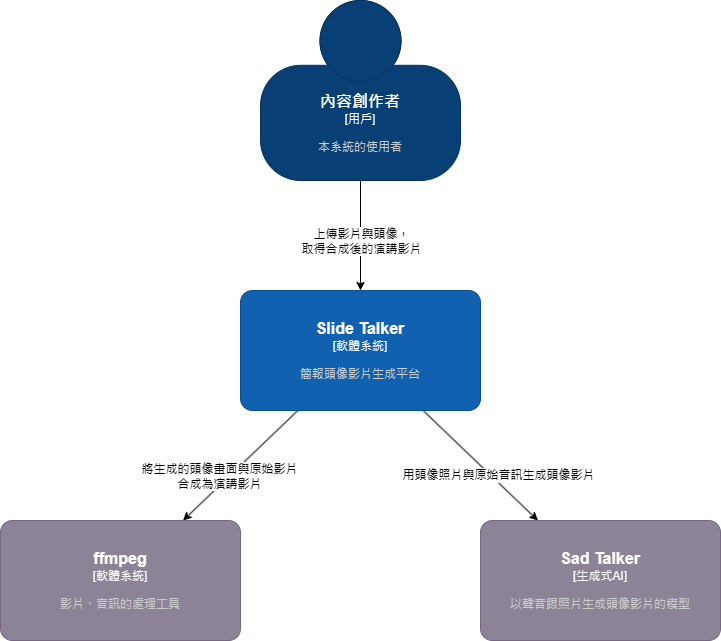
\includegraphics[width=.5\textwidth]{./ar0.png}
      % }
      \caption{Context Diagram}
      \label{ar0}
    \end{figure}
    \begin{figure}[H]
      \centering
      % \href{https://raw.githubusercontent.com/programingtw/proglearn-plan/main/img/testboard.png}{ 
        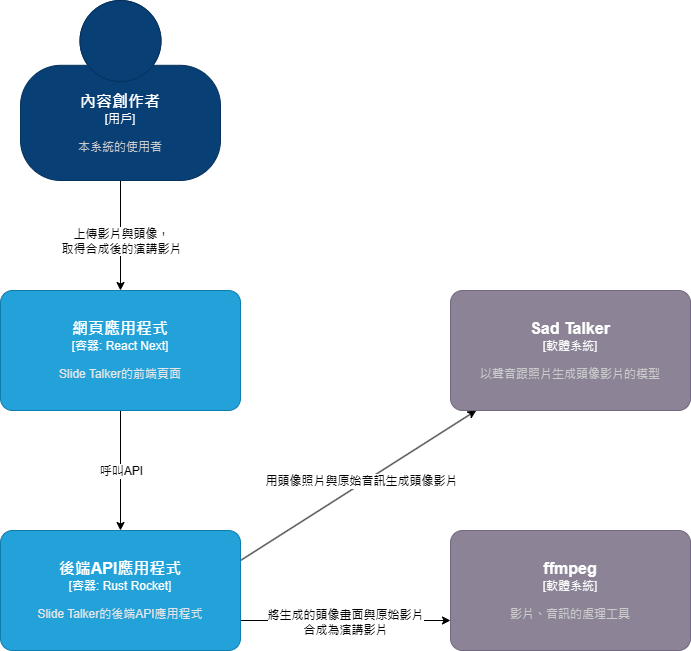
\includegraphics[width=.5\textwidth]{./ar1.png}
      % }
      \caption{Container Diagram}
      \label{ar1}
    \end{figure}
    \begin{figure}[H]
      \centering
      % \href{https://raw.githubusercontent.com/programingtw/proglearn-plan/main/img/testboard.png}{ 
        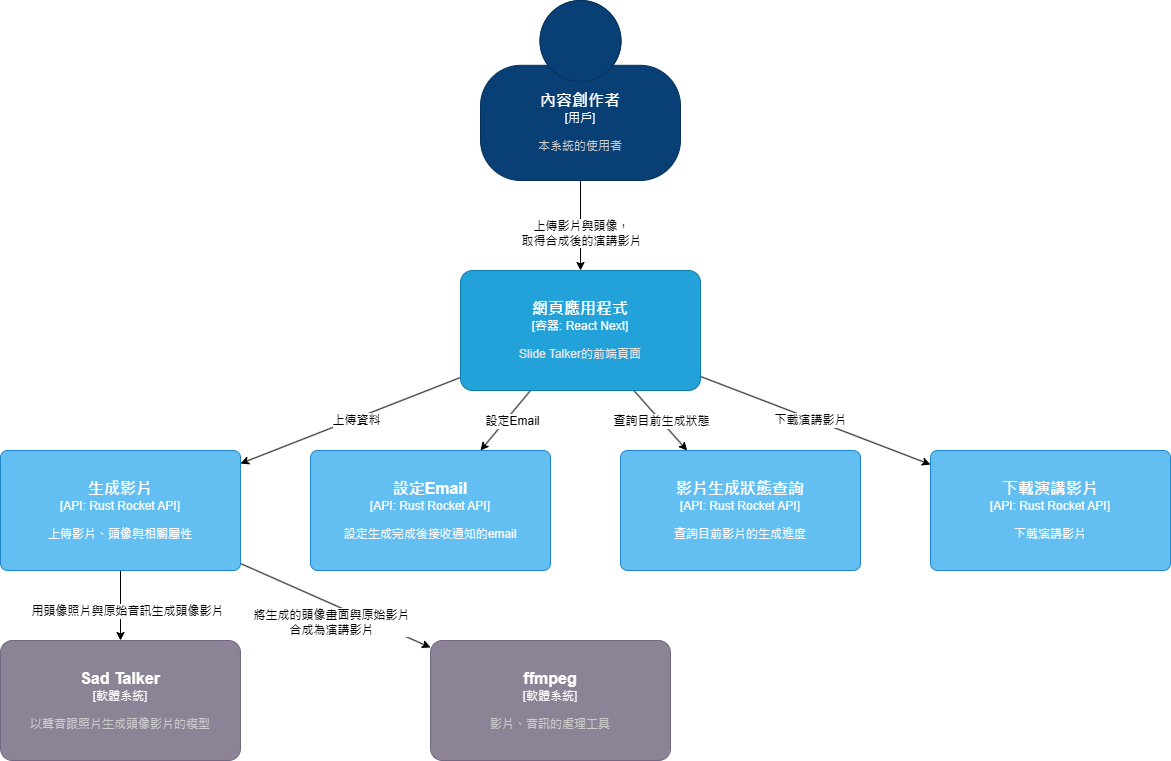
\includegraphics[width=.5\textwidth]{./ar2.png}
      % }
      \caption{Frontend Component Diagram}
      \label{ar2}
    \end{figure}
    \begin{figure}[H]
      \centering
      % \href{https://raw.githubusercontent.com/programingtw/proglearn-plan/main/img/testboard.png}{ 
        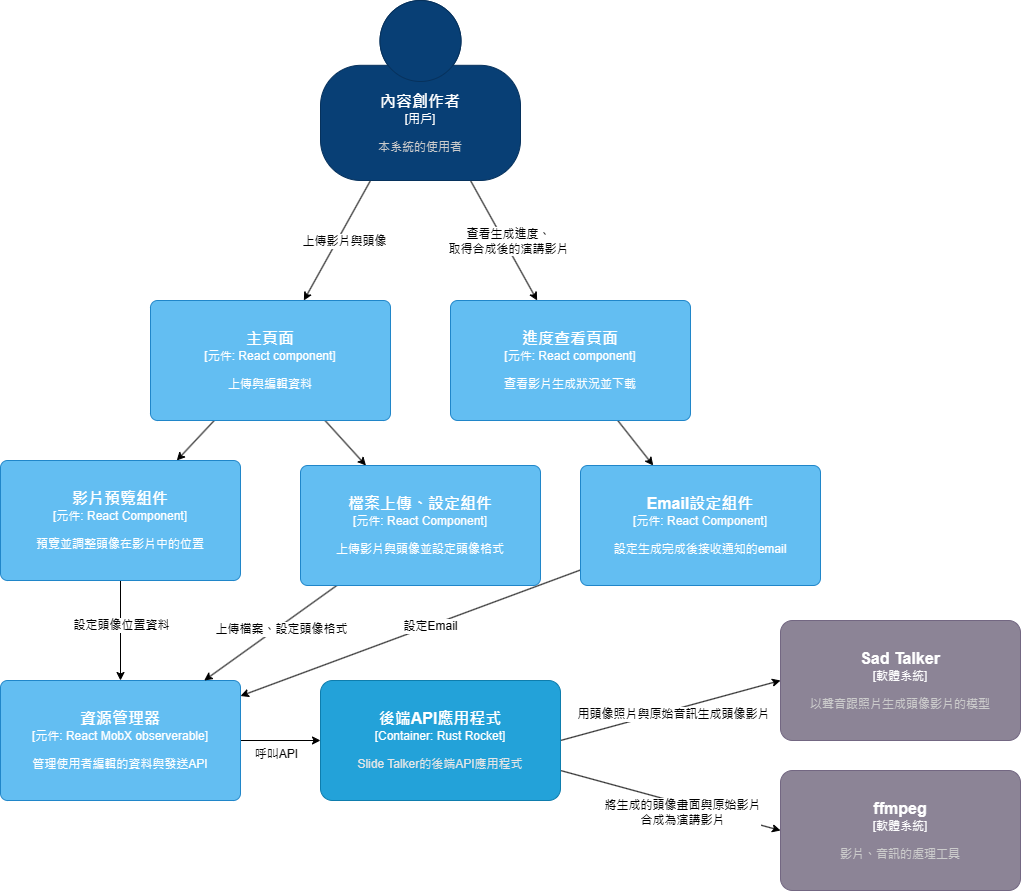
\includegraphics[width=.5\textwidth]{./ar3.png}
      % }
      \caption{Backend Component Diagram}
      \label{ar3}
    \end{figure}
  \item 開發技術介紹
    \begin{enumerate}
      \item 程式語言: TypeScript, Rust, Python
      \item 機器學習模型:Python,Python擁有龐大而活躍的機器學習生態系統,包括多個強大的函式庫和框架。
        \begin{enumerate}
          \item SadTalker\cite{sadtalker}: 音頻驅動的3D臉部說話動畫生成模型,用單一圖像作為輸入,並生成一個高度逼真的3D臉部動畫,能夠根據音頻信號進行表情和口型的變化,在逼真度和自然度上表現優異。
        \end{enumerate}
      \item 前端開發:React,用於構建用戶界面。它提供了組件化開發的方式,使得前端開發更加高效和可維護。
      \item 後端開發:Rust,使用Rust語言和Rocket框架來構建Web伺服器,提供後端支援。
    \end{enumerate}
  \item 作品展示
    \begin{figure}[H]
      \centering
      % \href{https://raw.githubusercontent.com/programingtw/proglearn-plan/main/img/testboard.png}{ 
        
\includegraphics[width=0.8\textwidth]{./s0.png}
      % }
      \caption{首頁}
      \label{s0}
    \end{figure}
    \begin{enumerate}[label=\arabic*.]
      \item 點選「開始創建」
    \end{enumerate}
    \begin{figure}[H]
      \centering
      % \href{https://raw.githubusercontent.com/programingtw/proglearn-plan/main/img/testboard.png}{ 
        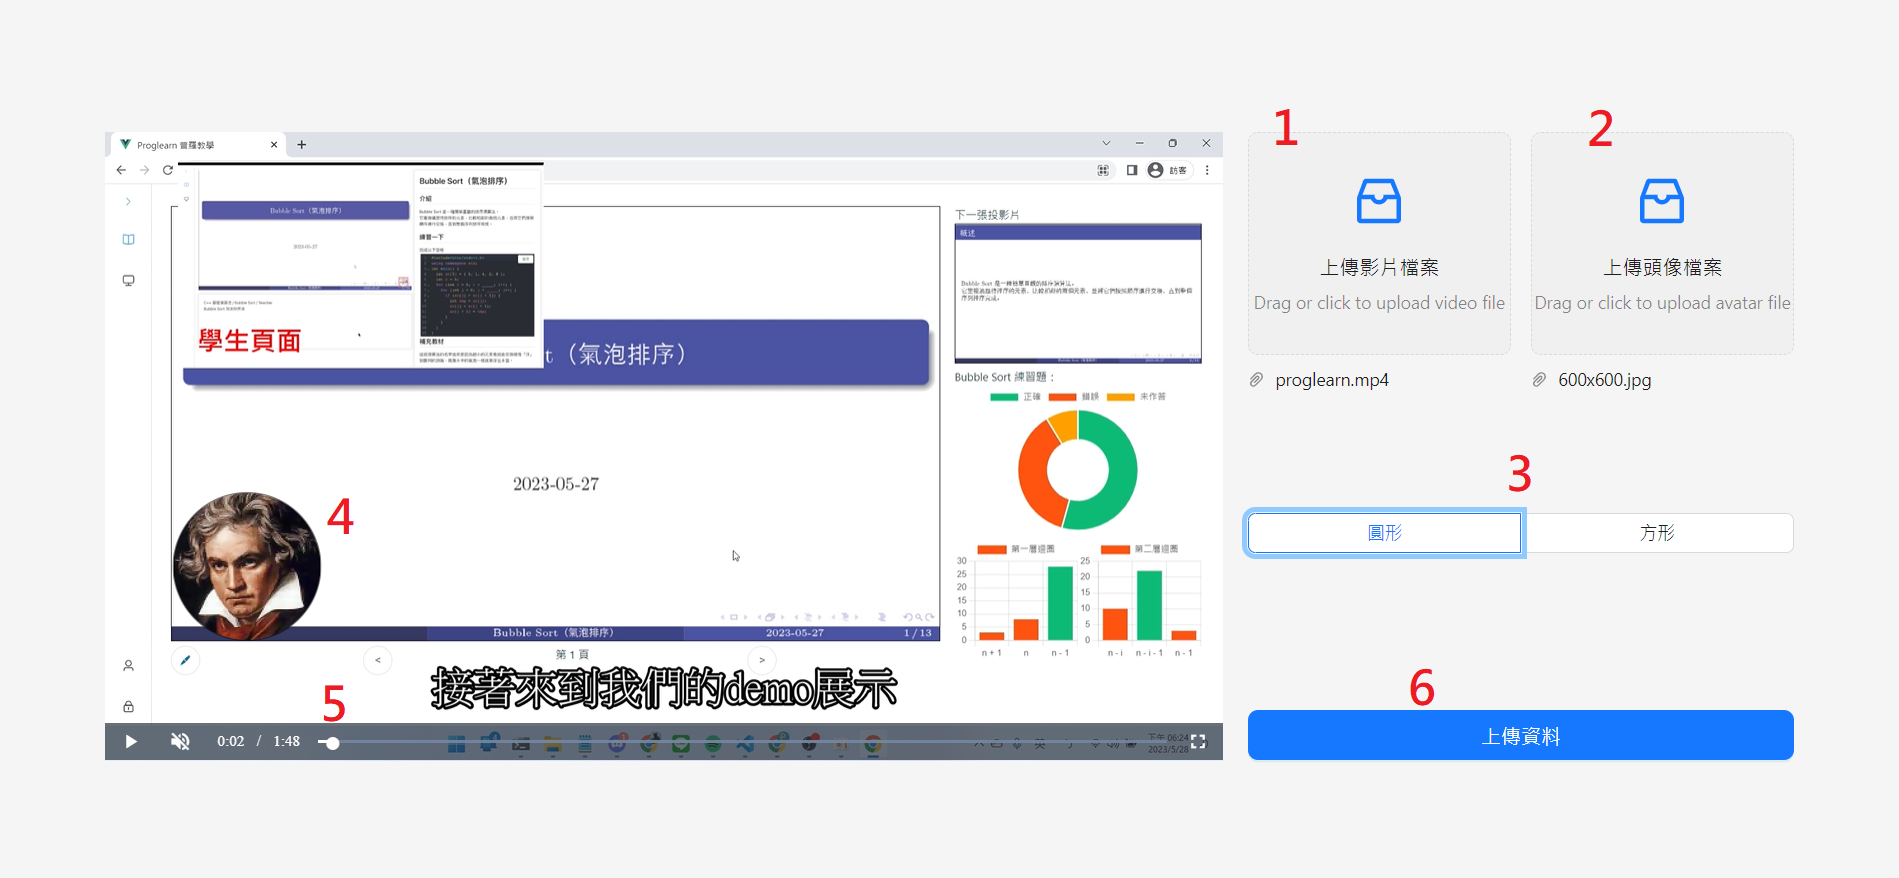
\includegraphics[width=0.8\textwidth]{./s1.png}
      % }
      \caption{合成設定頁}
      \label{s1}
    \end{figure}
    \begin{enumerate}[label=\arabic*.]
      \item 點選「上傳影片檔案」選擇影片
      \item 點選「上傳頭像檔案」選擇頭像照片
      \item 選擇頭相框的形狀(圓形、方形)
      \item 拖動畫面中頭像決定位置
      \item 拖拉影片時間軸檢視影片
      \item 點選「上傳資料」送出   
    \end{enumerate}
    \begin{figure}[H]
      \centering
      % \href{https://raw.githubusercontent.com/programingtw/proglearn-plan/main/img/testboard.png}{ 
        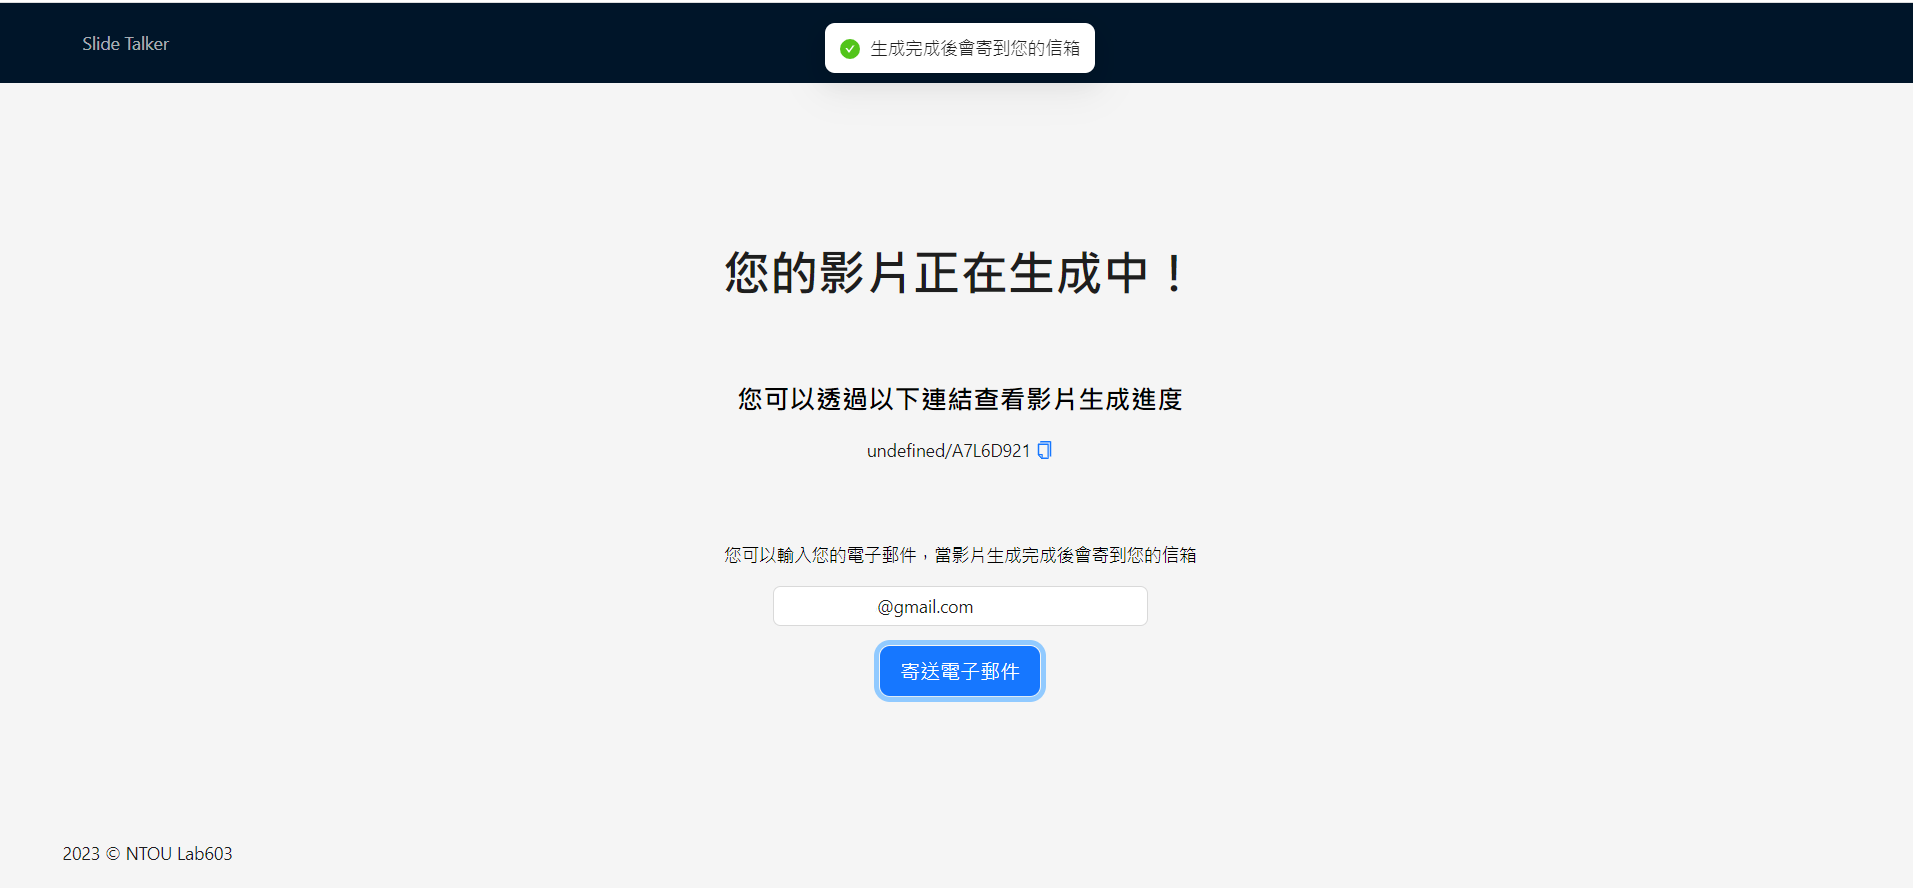
\includegraphics[width=0.8\textwidth]{./s2.png}
      % }
      \caption{影片查看進度頁面}
      \label{s2}
    \end{figure}
    \begin{figure}[H]
      \centering
      % \href{https://raw.githubusercontent.com/programingtw/proglearn-plan/main/img/testboard.png}{ 
        
\includegraphics[width=0.8\textwidth]{./s4.png}
      % }
      \caption{影片生成完成頁面}
      \label{s4}
    \end{figure}
    \begin{enumerate}[label=\arabic*.]
      \item 空格中輸入email並點選「寄送電子郵件」,影片完成後就會收到通知。
    \end{enumerate}
    \begin{figure}[H]
      \centering
      % \href{https://raw.githubusercontent.com/programingtw/proglearn-plan/main/img/testboard.png}{ 
        
\includegraphics[width=0.8\textwidth]{./s3.png}
      % }
      \caption{生成成功後的email 通知}
      \label{s3}
    \end{figure}
  \item 未來與展望
    \begin{enumerate}
      \item 改進機器學習模型:透過不斷優化和改進機器學習模型,可以提高生成頭部模擬影像的品質和逼真度,或是加入情緒的學習,使其更具人性化。
      \item 擴展功能:例如背景替換、虛擬道具或特效的添加,以提供更豐富和個性化的演講影片製作體驗。
      \item 雲端服務和即時處理:將作品部署到雲端平台,可以提供更高的可擴展性和效能,讓使用者能夠快速地上傳影片和照片並獲得即時的頭部模擬結果。
      \item 使用者互動和個性化:透過使用者的反饋和數據收集,可以進一步優化作品的使用者體驗。例如,根據使用者的偏好和需求,提供更多的個性化設定,讓使用者能夠自定義頭部模擬影像的風格或效果。
      \item 教學和培訓應用:除了演講影片,這個作品還可以應用於教學和培訓領域。透過頭部模擬影像的添加,可以增加教學影片的吸引力和互動性,提供更具教育價值的學習體驗。
    \end{enumerate}
  \item 參考文獻
    \renewcommand{\section}[2]{}
    \begin{thebibliography}{99}
      \bibitem{ref} Barbara Robertson, Mark J. Flowers, Determining the impact of lecture videos on student outcomes(2020)
      \bibitem{sadtalker}	SadTalker. Available from :  https://github.com/OpenTalker/SadTalker
    \end{thebibliography}
\end{enumerate}

\end{document}